% Options for packages loaded elsewhere
\PassOptionsToPackage{unicode}{hyperref}
\PassOptionsToPackage{hyphens}{url}
\PassOptionsToPackage{dvipsnames,svgnames,x11names}{xcolor}
%
\documentclass[
  letterpaper,
  DIV=11,
  numbers=noendperiod]{scrreport}

\usepackage{amsmath,amssymb}
\usepackage{lmodern}
\usepackage{iftex}
\ifPDFTeX
  \usepackage[T1]{fontenc}
  \usepackage[utf8]{inputenc}
  \usepackage{textcomp} % provide euro and other symbols
\else % if luatex or xetex
  \usepackage{unicode-math}
  \defaultfontfeatures{Scale=MatchLowercase}
  \defaultfontfeatures[\rmfamily]{Ligatures=TeX,Scale=1}
\fi
% Use upquote if available, for straight quotes in verbatim environments
\IfFileExists{upquote.sty}{\usepackage{upquote}}{}
\IfFileExists{microtype.sty}{% use microtype if available
  \usepackage[]{microtype}
  \UseMicrotypeSet[protrusion]{basicmath} % disable protrusion for tt fonts
}{}
\makeatletter
\@ifundefined{KOMAClassName}{% if non-KOMA class
  \IfFileExists{parskip.sty}{%
    \usepackage{parskip}
  }{% else
    \setlength{\parindent}{0pt}
    \setlength{\parskip}{6pt plus 2pt minus 1pt}}
}{% if KOMA class
  \KOMAoptions{parskip=half}}
\makeatother
\usepackage{xcolor}
\setlength{\emergencystretch}{3em} % prevent overfull lines
\setcounter{secnumdepth}{5}
% Make \paragraph and \subparagraph free-standing
\ifx\paragraph\undefined\else
  \let\oldparagraph\paragraph
  \renewcommand{\paragraph}[1]{\oldparagraph{#1}\mbox{}}
\fi
\ifx\subparagraph\undefined\else
  \let\oldsubparagraph\subparagraph
  \renewcommand{\subparagraph}[1]{\oldsubparagraph{#1}\mbox{}}
\fi


\providecommand{\tightlist}{%
  \setlength{\itemsep}{0pt}\setlength{\parskip}{0pt}}\usepackage{longtable,booktabs,array}
\usepackage{calc} % for calculating minipage widths
% Correct order of tables after \paragraph or \subparagraph
\usepackage{etoolbox}
\makeatletter
\patchcmd\longtable{\par}{\if@noskipsec\mbox{}\fi\par}{}{}
\makeatother
% Allow footnotes in longtable head/foot
\IfFileExists{footnotehyper.sty}{\usepackage{footnotehyper}}{\usepackage{footnote}}
\makesavenoteenv{longtable}
\usepackage{graphicx}
\makeatletter
\def\maxwidth{\ifdim\Gin@nat@width>\linewidth\linewidth\else\Gin@nat@width\fi}
\def\maxheight{\ifdim\Gin@nat@height>\textheight\textheight\else\Gin@nat@height\fi}
\makeatother
% Scale images if necessary, so that they will not overflow the page
% margins by default, and it is still possible to overwrite the defaults
% using explicit options in \includegraphics[width, height, ...]{}
\setkeys{Gin}{width=\maxwidth,height=\maxheight,keepaspectratio}
% Set default figure placement to htbp
\makeatletter
\def\fps@figure{htbp}
\makeatother

\usepackage{float}
\KOMAoption{captions}{tableheading}
\makeatletter
\makeatother
\makeatletter
\makeatother
\makeatletter
\@ifpackageloaded{caption}{}{\usepackage{caption}}
\AtBeginDocument{%
\ifdefined\contentsname
  \renewcommand*\contentsname{Table of contents}
\else
  \newcommand\contentsname{Table of contents}
\fi
\ifdefined\listfigurename
  \renewcommand*\listfigurename{List of Figures}
\else
  \newcommand\listfigurename{List of Figures}
\fi
\ifdefined\listtablename
  \renewcommand*\listtablename{List of Tables}
\else
  \newcommand\listtablename{List of Tables}
\fi
\ifdefined\figurename
  \renewcommand*\figurename{Figure}
\else
  \newcommand\figurename{Figure}
\fi
\ifdefined\tablename
  \renewcommand*\tablename{Table}
\else
  \newcommand\tablename{Table}
\fi
}
\@ifpackageloaded{float}{}{\usepackage{float}}
\floatstyle{ruled}
\@ifundefined{c@chapter}{\newfloat{codelisting}{h}{lop}}{\newfloat{codelisting}{h}{lop}[chapter]}
\floatname{codelisting}{Listing}
\newcommand*\listoflistings{\listof{codelisting}{List of Listings}}
\makeatother
\makeatletter
\@ifpackageloaded{caption}{}{\usepackage{caption}}
\@ifpackageloaded{subcaption}{}{\usepackage{subcaption}}
\makeatother
\makeatletter
\@ifpackageloaded{tcolorbox}{}{\usepackage[many]{tcolorbox}}
\makeatother
\makeatletter
\@ifundefined{shadecolor}{\definecolor{shadecolor}{rgb}{.97, .97, .97}}
\makeatother
\makeatletter
\makeatother
\ifLuaTeX
  \usepackage{selnolig}  % disable illegal ligatures
\fi
\IfFileExists{bookmark.sty}{\usepackage{bookmark}}{\usepackage{hyperref}}
\IfFileExists{xurl.sty}{\usepackage{xurl}}{} % add URL line breaks if available
\urlstyle{same} % disable monospaced font for URLs
\hypersetup{
  pdftitle={My Thesis},
  pdfauthor={Marziyeh S Jahromi},
  colorlinks=true,
  linkcolor={blue},
  filecolor={Maroon},
  citecolor={Blue},
  urlcolor={Blue},
  pdfcreator={LaTeX via pandoc}}

\title{My Thesis}
\usepackage{etoolbox}
\makeatletter
\providecommand{\subtitle}[1]{% add subtitle to \maketitle
  \apptocmd{\@title}{\par {\large #1 \par}}{}{}
}
\makeatother
\subtitle{STK analysis for GitHub}
\author{Marziyeh S Jahromi}
\date{11/16/23}

\begin{document}
\maketitle
\ifdefined\Shaded\renewenvironment{Shaded}{\begin{tcolorbox}[breakable, boxrule=0pt, enhanced, interior hidden, borderline west={3pt}{0pt}{shadecolor}, sharp corners, frame hidden]}{\end{tcolorbox}}\fi

\renewcommand*\contentsname{Table of contents}
{
\hypersetup{linkcolor=}
\setcounter{tocdepth}{2}
\tableofcontents
}
\hypertarget{introduction}{%
\chapter{Introduction}\label{introduction}}

\hypertarget{background}{%
\section{Background}\label{background}}

The Pamstation12 instrument provides a profiling of kinase activity of
cell or tissue samples. The device is loaded with either
serine/threonine or tyrosine microarray chips. Each chip has 4 wells so
four samples can be loaded on a single chip, and the Pamstation12 can
accommodate 3 chips per run. The microarray represents 144 (STK chip) or
196 (PTK chip) reporter peptides that can be phosphorylated by
serine/threonine or tyrosine kinases. The device measures the degree of
the phosphorylation in real time by detecting fluorescently labeled
antibodies at different exposure times. The list of peptides present in
each microarray can be viewed here:
\href{https://pamgene.com/wp-content/uploads/2020/09/STK-144-PamChip-87102.pdf}{STK
chip},
\href{https://pamgene.com/wp-content/uploads/2020/09/PTK-196-PamChip-86402.pdf}{PTK
chip}

\newpage

\begin{figure}[htbp]

{\centering 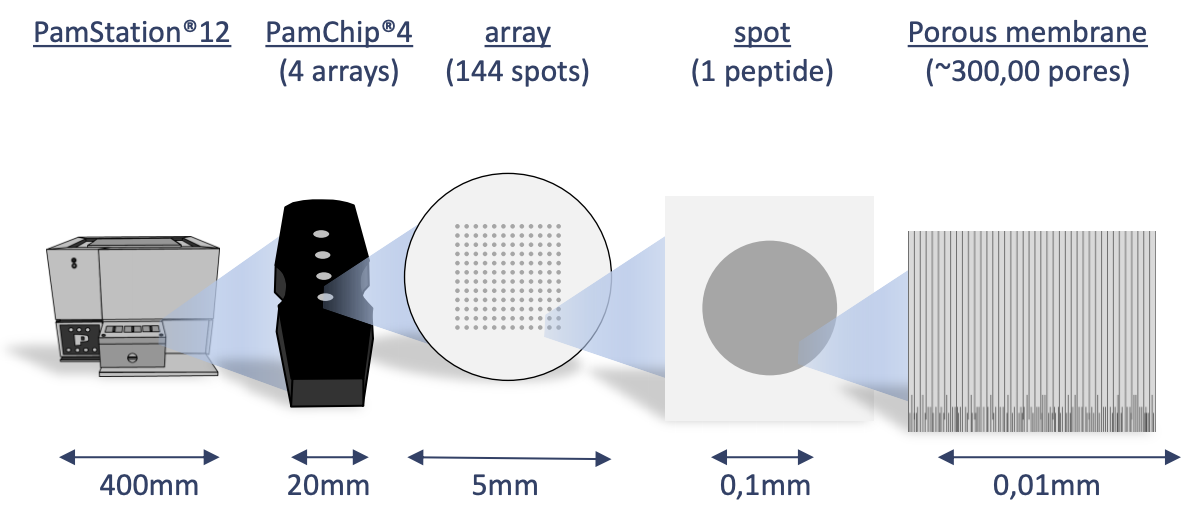
\includegraphics{images/pamgene_workflow.png}

}

\caption{Pamgene Kinase Activity Platform}

\end{figure}

\begin{figure}[htbp]

{\centering 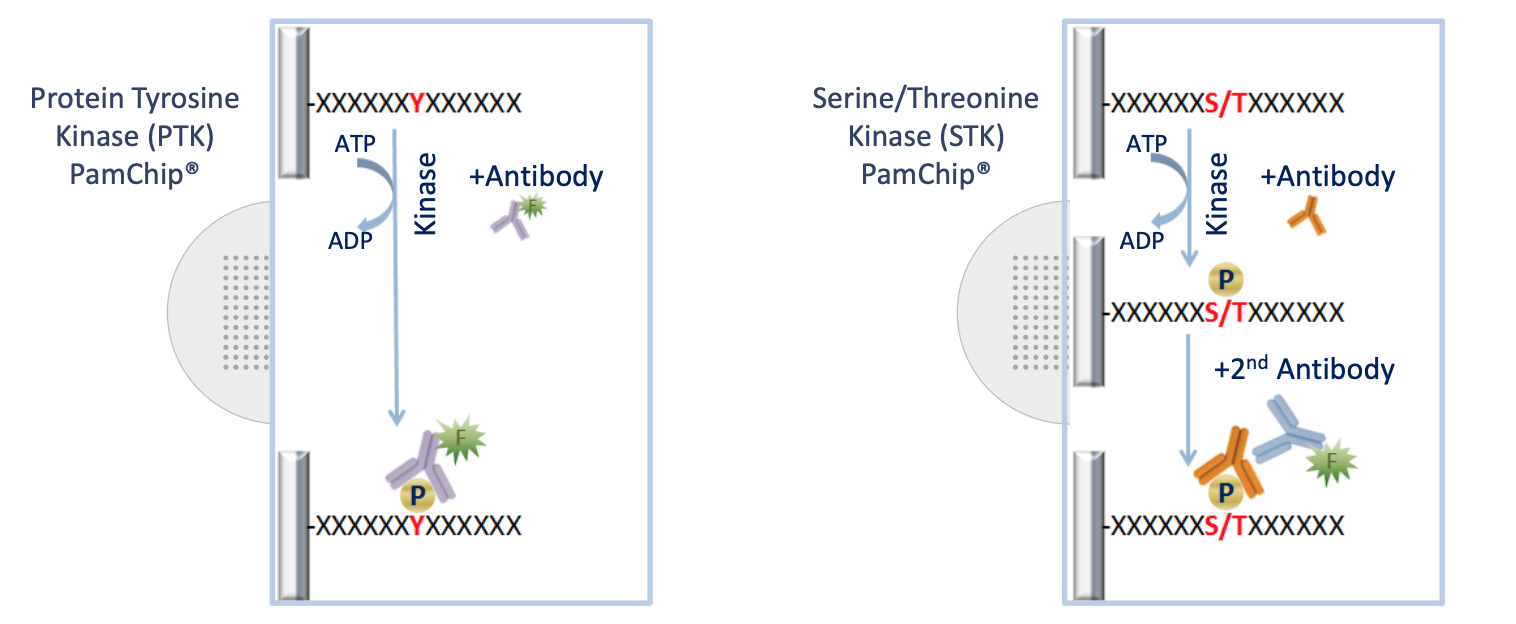
\includegraphics{images/pamgene_detectionFig.png}

}

\caption{Pamgene Platform Detection}

\end{figure}

\hypertarget{run-design}{%
\chapter{Run Design}\label{run-design}}

Designing the placement of the samples on the chips and arrays is
important to consider due to the variability across different chips and
batches. During the run some wells are subject to fail and their data
cannot be analyzed and shown below as red.

\begin{figure}[htbp]

{\centering \includegraphics{template_files/figure-pdf/design-1.pdf}

}

\end{figure}

\hypertarget{results}{%
\chapter{Results}\label{results}}

\hypertarget{image-analysis}{%
\section{Image Analysis}\label{image-analysis}}

The first step of analyzing the run is to convert the images taken by
the PamStation of each array at different exposure times to numerical
values This is done by the Bionavigator software developed by Pamgene.
The software recognizes the grid of the array with the aid of the
searching algorithm (Pamgrid) to correctly identify each spot on the
array. The numbers produced by this software represent the median value
of the foreground pixels minus the median value of the background pixels
to produce the median signal minus background (Median\_SigmBg).

\hypertarget{reading-data}{%
\section{Reading Data}\label{reading-data}}

The first step will be reading the crosstab view bionavigator files
(Median\_SigmBg and Signal\_Saturation) and defining the PamChip type
(STK or PTK). The raw data is read and then transformed to be in tidy
format for an easier analysis, modeling, and visualizing.

\hypertarget{qc-initial-steps-and-groups-assignments}{%
\section{QC Initial Steps and Groups
Assignments}\label{qc-initial-steps-and-groups-assignments}}

We will perform a couple of quality control steps to deal with negative
values in the data and adjust based on signal saturation (optional).
Next, we will define a new column to represent the grouping. And then,
we will extract end point signal values

\hypertarget{qc-steps-and-model-fitting}{%
\section{QC Steps and Model Fitting}\label{qc-steps-and-model-fitting}}

We will filter out peptides with low signals. In order to combine the
values from different exposure times into a single value, a simple
linear regression model of the \emph{Median\_SigmBg} as a function of
exposure time is fitted. The slope of of the model fit and \(R^2\) are
then used for quality control and samples comparison. The slope is also
scaled by multiplying by 100 and log2 transformed
(\emph{Slope\_Transformed}). We then filter out peptides with poor
linear fit and references peptides.

\hypertarget{global-signal-intensity}{%
\section{Global Signal Intensity}\label{global-signal-intensity}}

For a global signal intensity across all samples/groups, few figures can
be plotted based on the \emph{Slope\_Transformed} values.

\hypertarget{global-cv-plots}{%
\subsection{Global CV Plots}\label{global-cv-plots}}

We will plot the coefficient of variation on both the normal and
normalized fits. This will help us to identify groups with high
variation that could be explained by sample outliers.

\begin{figure}[htbp]

{\centering \includegraphics{template_files/figure-pdf/global-cv-plot-1.pdf}

}

\caption{Coefficient of Variation plotted for each peptide across all 4
groups}

\end{figure}

\hypertarget{global-violin-plots}{%
\subsection{Global Violin Plots}\label{global-violin-plots}}

We will plot violin figures to examine global signal differences between
groups/samples.

\begin{figure}[htbp]

{\centering \includegraphics{template_files/figure-pdf/global-violin-plot-by-group-1.pdf}

}

\caption{Violin Plots for signal intensity Distribution Across Groups
for all replicates}

\end{figure}

\begin{figure}[htbp]

{\centering \includegraphics{template_files/figure-pdf/global-violin-plot-by-chip-1.pdf}

}

\caption{Violin Plots for signal intensity Distribution Across Chips for
all replicates}

\end{figure}

\hypertarget{global-heatmaps}{%
\subsection{Global Heatmaps}\label{global-heatmaps}}

The heatmap represent all the peptides present on the chip except the
positive/internal controls and peptides that failed to pass QC. The
heatmaps are scaled by row to highlight the peptide signal differences
across the samples. A hierarchical unsupervised clustering is applied
both on the peptides and the samples to group potentially similar
signatures.

\begin{figure}[htbp]

{\centering \includegraphics{template_files/figure-pdf/global-signal-heatmap-individual-1.pdf}

}

\caption{Row and chip normalized intensity values for the selected
peptides}

\end{figure}

\begin{figure}[htbp]

{\centering \includegraphics{template_files/figure-pdf/global-signal-heatmap-grouped-1.pdf}

}

\caption{Row and group normalized intensity values for the selected
peptides}

\end{figure}

\hypertarget{group-comparison}{%
\section{Group Comparison}\label{group-comparison}}

To compare between samples, a two-group comparison is performed. In this
case, there are three group comparisons:

\begin{itemize}
\tightlist
\item
  AMPK KD Neuron + Untreated vs Wild Type Neuron + AICAR
\item
  AMPK KD Neuron + Untreated vs Wild Type Neuron + Untreated
\item
  AMPK KD Neuron + AICAR vs Wild Type Neuron + AICAR
\end{itemize}

The \emph{Slope\_Transformed} ratio between each group, paired by chip,
is calculated to the fold change. Based on the fold change, peptides
that pass a certain fold change threshold are considered significant
hits. Also, quality control steps applied in each comparison to filter
out peptides that do not reach specific criteria:

\begin{itemize}
\tightlist
\item
  The \emph{Median\_SigmBg} at max exposure \emph{100ms} must be above a
  certain value\\
\item
  \(R^2\) of the linear model fit must be above a threshold value
\end{itemize}

These \emph{Filtering Parameters} (fold change threshold, QC criteria)
can be modified to adjust the stringency of the analysis. The
\emph{Filtering Parameters} that are used for this analysis:

\begin{itemize}
\tightlist
\item
  The \emph{Median\_SigmBg} at max exposure \emph{100ms} must be equal
  or above 5\\
\item
  \(R^2\) of the linear model fit must be above or equal 0.8\\
\item
  Log fold change (LFC) cutoffs at (0.2,0.3,0.4)
\end{itemize}

\begin{figure}[htbp]

{\centering \includegraphics{template_files/figure-pdf/childA-1.pdf}

}

\end{figure}

\hypertarget{male_ins-vs-male_veh}{%
\subsection{Male\_INS vs Male\_VEH}\label{male_ins-vs-male_veh}}

\hypertarget{heatmap}{%
\subsubsection{Heatmap}\label{heatmap}}

After applying the \emph{Filtering Parameters} for this group
comparison, only \emph{33}/141 peptides carried forward in the analysis
(i.e.~\emph{33 hits}). Below are some figures to visualize the
differences between these samples for considering these \emph{hits}.

\hypertarget{violin-plot}{%
\subsubsection{Violin Plot}\label{violin-plot}}

Below, the violin plot visualizes the distribution of selected peptides
for the analysis.

\begin{figure}[htbp]

{\centering \includegraphics{template_files/figure-pdf/violinIndPlotA-1.pdf}

}

\caption{Violin plot of two groups}

\end{figure}

\hypertarget{waterfall-plot}{%
\subsubsection{Waterfall Plot}\label{waterfall-plot}}

This waterfall represents the log2 fold changes between the two groups
at each peptide.

\begin{figure}[htbp]

{\centering \includegraphics{template_files/figure-pdf/waterfallA-1.pdf}

}

\caption{Waterfall Plot to show the distribution of change in peptide
phosphorylation}

\end{figure}

\hypertarget{upstream-kinase-analysis}{%
\subsubsection{Upstream Kinase
Analysis}\label{upstream-kinase-analysis}}

The lab carefully curated and mapped the kinases that can act and
phosphorylate each peptide present on the chip. This was achieved by
using multiple sources including GPS 3.0, Kinexus Phosphonet, PhosphoELM
and PhosphoSite Plus. Based on that association between peptides and
kinases, a random sampling analysis is performed for these hits. The
basic idea of \emph{KRSA} is: For each iteration (\emph{2000} iterations
performed in this analysis), the same number of hits are randomly
selected from the total 141/or 193 peptides present on the chip.
Predicted kinases are then mapped to this sample list of peptides and
number of kinases are determined. The kinase count from the actual hits
and random sampling is then compared to determine the significance.

\begin{longtable}[]{@{}lr@{}}
\toprule()
Kinase & AvgZ \\
\midrule()
\endhead
CHK1 & 1.9100000 \\
DYRK & 1.8966667 \\
MST & 1.7608333 \\
BRSK & 1.6058333 \\
P38 & 1.5125000 \\
VRK1 & 1.4366667 \\
KHS & 1.4041667 \\
JNK & 1.2366667 \\
MARK & 1.1408333 \\
MAPKAPK & 1.1250000 \\
CK1 & -0.8116667 \\
CAMK2 & -0.8275000 \\
PKCD & -0.8291667 \\
PAKA & -0.8300000 \\
NMO & -0.8875000 \\
STE11 & -0.9691667 \\
PKA & -1.2216667 \\
RIPK & -1.3450000 \\
PLK & -1.5150000 \\
PKD & -1.8191667 \\
\bottomrule()
\end{longtable}

\begin{longtable}[]{@{}lr@{}}
\toprule()
Method & NumberOfPeptides \\
\midrule()
\endhead
meanLFC.0.15 & 39 \\
meanLFC.0.2 & 33 \\
meanLFC.0.3 & 19 \\
meanLFC.0.4 & 15 \\
710429119.0.15 & 24 \\
710429119.0.2 & 21 \\
710429119.0.3 & 16 \\
710429119.0.4 & 11 \\
710429120.0.15 & 37 \\
710429120.0.2 & 29 \\
710429120.0.3 & 16 \\
710429120.0.4 & 9 \\
710429121.0.15 & 57 \\
710429121.0.2 & 53 \\
710429121.0.3 & 47 \\
710429121.0.4 & 37 \\
\bottomrule()
\end{longtable}

\hypertarget{z-scores-plot}{%
\subsubsection{Z Scores Plot}\label{z-scores-plot}}

We will plot the individual and averaged Z scores using both the across
and within chip analyses.

\begin{figure}[htbp]

{\centering \includegraphics{template_files/figure-pdf/zscoresPlotA-1.pdf}

}

\caption{Waterfall plot of the Z Scores of each kinase family}

\end{figure}

\hypertarget{reverse-krsa-plot}{%
\subsubsection{Reverse KRSA Plot}\label{reverse-krsa-plot}}

We will use the reverse KRSA plot function, to plot the log2 fold change
values for all peptides mapped to kinase hits. This will help us examine
the activity of the kinase

\begin{figure}[htbp]

{\centering \includegraphics{template_files/figure-pdf/revKRSAPlotA-1.pdf}

}

\caption{Kinase Activity summary for each kinase family based on peptide
phsophorylation}

\end{figure}

\hypertarget{coverage-plot}{%
\subsubsection{Coverage Plot}\label{coverage-plot}}

To view the coverage of kinases across the full list of peptides on the
chip, we will use the coverage plot function

\begin{figure}[htbp]

{\centering \includegraphics{template_files/figure-pdf/covPlotA-1.pdf}

}

\caption{Percentge of peptides each kinase family phosphorylates}

\end{figure}

\hypertarget{ball-model-network}{%
\subsubsection{Ball Model Network}\label{ball-model-network}}

We will view the ball model network function, to generate a model
representing the protein-protein interactions between kinases

\begin{figure}[htbp]

{\centering \includegraphics{template_files/figure-pdf/netPlotA-1.pdf}

}

\end{figure}

\newpage

\begin{figure}[htbp]

{\centering \includegraphics{template_files/figure-pdf/childB-1.pdf}

}

\end{figure}

\hypertarget{female_ins-vs-female_veh}{%
\subsection{Female\_INS vs Female\_VEH}\label{female_ins-vs-female_veh}}

\hypertarget{heatmap-1}{%
\subsubsection{Heatmap}\label{heatmap-1}}

After applying the \emph{Filtering Parameters} for this group
comparison, only \emph{37}/141 peptides carried forward in the analysis
(i.e.~\emph{37 hits}). Below are some figures to visualize the
differences between these samples for considering these \emph{hits}.

\hypertarget{violin-plot-1}{%
\subsubsection{Violin Plot}\label{violin-plot-1}}

Below, the violin plot visualizes the distribution of selected peptides
for the analysis.

\begin{figure}[htbp]

{\centering \includegraphics{template_files/figure-pdf/violinIndPlotB-1.pdf}

}

\caption{Violin plot of two groups}

\end{figure}

\hypertarget{waterfall-plot-1}{%
\subsubsection{Waterfall Plot}\label{waterfall-plot-1}}

This waterfall represents the log2 fold changes between the two groups
at each peptide.

\begin{figure}[htbp]

{\centering \includegraphics{template_files/figure-pdf/waterfallB-1.pdf}

}

\caption{Waterfall Plot to show the distribution of change in peptide
phosphorylation}

\end{figure}

\hypertarget{upstream-kinase-analysis-1}{%
\subsubsection{Upstream Kinase
Analysis}\label{upstream-kinase-analysis-1}}

The lab carefully curated and mapped the kinases that can act and
phosphorylate each peptide present on the chip. This was achieved by
using multiple sources including GPS 3.0, Kinexus Phosphonet, PhosphoELM
and PhosphoSite Plus. Based on that association between peptides and
kinases, a random sampling analysis is performed for these hits. The
basic idea of \emph{KRSA} is: For each iteration (\emph{2000} iterations
performed in this analysis), the same number of hits are randomly
selected from the total 141/or 193 peptides present on the chip.
Predicted kinases are then mapped to this sample list of peptides and
number of kinases are determined. The kinase count from the actual hits
and random sampling is then compared to determine the significance.

\begin{longtable}[]{@{}lr@{}}
\toprule()
Kinase & AvgZ \\
\midrule()
\endhead
ERK & 2.684167 \\
VRK1 & 2.673333 \\
MLCK & 2.275000 \\
PKN & 1.958333 \\
PKCH & 1.850000 \\
P38 & 1.677500 \\
JNK & 1.625000 \\
DYRK & 1.412500 \\
MLK & 1.255000 \\
MST & 1.164167 \\
PKCD & -1.108333 \\
STE11 & -1.118333 \\
NMO & -1.197500 \\
RIPK & -1.203333 \\
RSK & -1.270833 \\
PLK & -1.298333 \\
PHK & -1.439167 \\
PKG & -1.561667 \\
PKD & -1.833333 \\
PKA & -2.137500 \\
\bottomrule()
\end{longtable}

\begin{longtable}[]{@{}lr@{}}
\toprule()
Method & NumberOfPeptides \\
\midrule()
\endhead
meanLFC.0.15 & 43 \\
meanLFC.0.2 & 37 \\
meanLFC.0.3 & 31 \\
meanLFC.0.4 & 23 \\
710429119.0.15 & 42 \\
710429119.0.2 & 41 \\
710429119.0.3 & 32 \\
710429119.0.4 & 24 \\
710429120.0.15 & 42 \\
710429120.0.2 & 40 \\
710429120.0.3 & 30 \\
710429120.0.4 & 22 \\
710429121.0.15 & 42 \\
710429121.0.2 & 39 \\
710429121.0.3 & 31 \\
710429121.0.4 & 23 \\
\bottomrule()
\end{longtable}

\hypertarget{z-scores-plot-1}{%
\subsubsection{Z Scores Plot}\label{z-scores-plot-1}}

We will plot the individual and averaged Z scores using both the across
and within chip analyses.

\begin{figure}[htbp]

{\centering \includegraphics{template_files/figure-pdf/zscoresPlotB-1.pdf}

}

\caption{Waterfall plot of the Z Scores of each kinase family}

\end{figure}

\hypertarget{reverse-krsa-plot-1}{%
\subsubsection{Reverse KRSA Plot}\label{reverse-krsa-plot-1}}

We will use the reverse KRSA plot function, to plot the log2 fold change
values for all peptides mapped to kinase hits. This will help us examine
the activity of the kinase

\begin{figure}[htbp]

{\centering \includegraphics{template_files/figure-pdf/revKRSAPlotB-1.pdf}

}

\caption{Kinase Activity summary for each kinase family based on peptide
phsophorylation}

\end{figure}

\hypertarget{coverage-plot-1}{%
\subsubsection{Coverage Plot}\label{coverage-plot-1}}

To view the coverage of kinases across the full list of peptides on the
chip, we will use the coverage plot function

\begin{figure}[htbp]

{\centering \includegraphics{template_files/figure-pdf/covPlotB-1.pdf}

}

\caption{Percentge of peptides each kinase family phosphorylates}

\end{figure}

\hypertarget{ball-model-network-1}{%
\subsubsection{Ball Model Network}\label{ball-model-network-1}}

We will view the ball model network function, to generate a model
representing the protein-protein interactions between kinases

\begin{figure}[htbp]

{\centering \includegraphics{template_files/figure-pdf/netPlotB-1.pdf}

}

\end{figure}

\newpage

\begin{figure}[htbp]

{\centering \includegraphics{template_files/figure-pdf/childC-1.pdf}

}

\end{figure}

\hypertarget{male_veh-vs-female_veh}{%
\subsection{Male\_VEH vs Female\_VEH}\label{male_veh-vs-female_veh}}

\hypertarget{heatmap-2}{%
\subsubsection{Heatmap}\label{heatmap-2}}

After applying the \emph{Filtering Parameters} for this group
comparison, only \emph{35}/141 peptides carried forward in the analysis
(i.e.~\emph{35 hits}). Below are some figures to visualize the
differences between these samples for considering these \emph{hits}.

\hypertarget{violin-plot-2}{%
\subsubsection{Violin Plot}\label{violin-plot-2}}

Below, the violin plot visualizes the distribution of selected peptides
for the analysis.

\begin{figure}[htbp]

{\centering \includegraphics{template_files/figure-pdf/violinIndPlotC-1.pdf}

}

\caption{Violin plot of two groups}

\end{figure}

\hypertarget{waterfall-plot-2}{%
\subsubsection{Waterfall Plot}\label{waterfall-plot-2}}

This waterfall represents the log2 fold changes between the two groups
at each peptide.

\begin{figure}[htbp]

{\centering \includegraphics{template_files/figure-pdf/waterfallC-1.pdf}

}

\caption{Waterfall Plot to show the distribution of change in peptide
phosphorylation}

\end{figure}

\hypertarget{upstream-kinase-analysis-2}{%
\subsubsection{Upstream Kinase
Analysis}\label{upstream-kinase-analysis-2}}

The lab carefully curated and mapped the kinases that can act and
phosphorylate each peptide present on the chip. This was achieved by
using multiple sources including GPS 3.0, Kinexus Phosphonet, PhosphoELM
and PhosphoSite Plus. Based on that association between peptides and
kinases, a random sampling analysis is performed for these hits. The
basic idea of \emph{KRSA} is: For each iteration (\emph{2000} iterations
performed in this analysis), the same number of hits are randomly
selected from the total 141/or 193 peptides present on the chip.
Predicted kinases are then mapped to this sample list of peptides and
number of kinases are determined. The kinase count from the actual hits
and random sampling is then compared to determine the significance.

\begin{longtable}[]{@{}lr@{}}
\toprule()
Kinase & AvgZ \\
\midrule()
\endhead
PAKB & 2.3666667 \\
AKT & 2.1683333 \\
SGK & 1.9583333 \\
MST & 1.9466667 \\
MAPKAPK & 1.8716667 \\
CHK1 & 1.8316667 \\
TAO & 1.7941667 \\
KHS & 1.7791667 \\
P38 & 1.6225000 \\
CDK & 1.4741667 \\
GSK & -0.7750000 \\
TLK & -0.8166667 \\
STE7 & -0.8416667 \\
RIPK & -1.1566667 \\
PLK & -1.1766667 \\
AUR & -1.2216667 \\
STE11 & -1.2366667 \\
PKD & -1.2400000 \\
PKCD & -1.3683333 \\
NMO & -1.7116667 \\
\bottomrule()
\end{longtable}

\begin{longtable}[]{@{}lr@{}}
\toprule()
Method & NumberOfPeptides \\
\midrule()
\endhead
meanLFC.0.15 & 47 \\
meanLFC.0.2 & 35 \\
meanLFC.0.3 & 26 \\
meanLFC.0.4 & 21 \\
710429119.0.15 & 39 \\
710429119.0.2 & 32 \\
710429119.0.3 & 24 \\
710429119.0.4 & 20 \\
710429120.0.15 & 42 \\
710429120.0.2 & 38 \\
710429120.0.3 & 28 \\
710429120.0.4 & 24 \\
710429121.0.15 & 55 \\
710429121.0.2 & 51 \\
710429121.0.3 & 42 \\
710429121.0.4 & 32 \\
\bottomrule()
\end{longtable}

\hypertarget{z-scores-plot-2}{%
\subsubsection{Z Scores Plot}\label{z-scores-plot-2}}

We will plot the individual and averaged Z scores using both the across
and within chip analyses.

\begin{figure}[htbp]

{\centering \includegraphics{template_files/figure-pdf/zscoresPlotC-1.pdf}

}

\caption{Waterfall plot of the Z Scores of each kinase family}

\end{figure}

\hypertarget{reverse-krsa-plot-2}{%
\subsubsection{Reverse KRSA Plot}\label{reverse-krsa-plot-2}}

We will use the reverse KRSA plot function, to plot the log2 fold change
values for all peptides mapped to kinase hits. This will help us examine
the activity of the kinase

\begin{figure}[htbp]

{\centering \includegraphics{template_files/figure-pdf/revKRSAPlotC-1.pdf}

}

\caption{Kinase Activity summary for each kinase family based on peptide
phsophorylation}

\end{figure}

\hypertarget{coverage-plot-2}{%
\subsubsection{Coverage Plot}\label{coverage-plot-2}}

To view the coverage of kinases across the full list of peptides on the
chip, we will use the coverage plot function

\begin{figure}[htbp]

{\centering \includegraphics{template_files/figure-pdf/covPlotC-1.pdf}

}

\caption{Percentge of peptides each kinase family phosphorylates}

\end{figure}

\hypertarget{ball-model-network-2}{%
\subsubsection{Ball Model Network}\label{ball-model-network-2}}

We will view the ball model network function, to generate a model
representing the protein-protein interactions between kinases

\begin{figure}[htbp]

{\centering \includegraphics{template_files/figure-pdf/netPlotC-1.pdf}

}

\end{figure}

\newpage

\begin{figure}[htbp]

{\centering \includegraphics{template_files/figure-pdf/childD-1.pdf}

}

\end{figure}

\hypertarget{male_ins-vs-female_ins}{%
\subsection{Male\_INS vs Female\_INS}\label{male_ins-vs-female_ins}}

\hypertarget{heatmap-3}{%
\subsubsection{Heatmap}\label{heatmap-3}}

After applying the \emph{Filtering Parameters} for this group
comparison, only \emph{46}/141 peptides carried forward in the analysis
(i.e.~\emph{46 hits}). Below are some figures to visualize the
differences between these samples for considering these \emph{hits}.

\hypertarget{violin-plot-3}{%
\subsubsection{Violin Plot}\label{violin-plot-3}}

Below, the violin plot visualizes the distribution of selected peptides
for the analysis.

\begin{figure}[htbp]

{\centering \includegraphics{template_files/figure-pdf/violinIndPlotD-1.pdf}

}

\caption{Violin plot of two groups}

\end{figure}

\hypertarget{waterfall-plot-3}{%
\subsubsection{Waterfall Plot}\label{waterfall-plot-3}}

This waterfall represents the log2 fold changes between the two groups
at each peptide.

\begin{figure}[htbp]

{\centering \includegraphics{template_files/figure-pdf/waterfallD-1.pdf}

}

\caption{Waterfall Plot to show the distribution of change in peptide
phosphorylation}

\end{figure}

\hypertarget{upstream-kinase-analysis-3}{%
\subsubsection{Upstream Kinase
Analysis}\label{upstream-kinase-analysis-3}}

The lab carefully curated and mapped the kinases that can act and
phosphorylate each peptide present on the chip. This was achieved by
using multiple sources including GPS 3.0, Kinexus Phosphonet, PhosphoELM
and PhosphoSite Plus. Based on that association between peptides and
kinases, a random sampling analysis is performed for these hits. The
basic idea of \emph{KRSA} is: For each iteration (\emph{2000} iterations
performed in this analysis), the same number of hits are randomly
selected from the total 141/or 193 peptides present on the chip.
Predicted kinases are then mapped to this sample list of peptides and
number of kinases are determined. The kinase count from the actual hits
and random sampling is then compared to determine the significance.

\begin{longtable}[]{@{}lr@{}}
\toprule()
Kinase & AvgZ \\
\midrule()
\endhead
ERK & 2.786667 \\
VRK1 & 2.484167 \\
MLCK & 2.220000 \\
PKN & 2.140833 \\
MST & 2.036667 \\
P38 & 1.919167 \\
DYRK & 1.695000 \\
PKCH & 1.580000 \\
CHK1 & 1.551667 \\
BUD32 & 1.210000 \\
MTOR & -1.008333 \\
CK1 & -1.064167 \\
PLK & -1.089167 \\
NEK & -1.095000 \\
CAMK2 & -1.273333 \\
PKA & -1.354167 \\
RIPK & -1.450000 \\
STE11 & -1.545000 \\
NMO & -1.645000 \\
PKD & -2.070000 \\
\bottomrule()
\end{longtable}

\begin{longtable}[]{@{}lr@{}}
\toprule()
Method & NumberOfPeptides \\
\midrule()
\endhead
meanLFC.0.15 & 51 \\
meanLFC.0.2 & 46 \\
meanLFC.0.3 & 44 \\
meanLFC.0.4 & 29 \\
710429119.0.15 & 51 \\
710429119.0.2 & 49 \\
710429119.0.3 & 46 \\
710429119.0.4 & 40 \\
710429120.0.15 & 49 \\
710429120.0.2 & 47 \\
710429120.0.3 & 38 \\
710429120.0.4 & 28 \\
710429121.0.15 & 42 \\
710429121.0.2 & 36 \\
710429121.0.3 & 29 \\
710429121.0.4 & 24 \\
\bottomrule()
\end{longtable}

\hypertarget{z-scores-plot-3}{%
\subsubsection{Z Scores Plot}\label{z-scores-plot-3}}

We will plot the individual and averaged Z scores using both the across
and within chip analyses.

\begin{figure}[htbp]

{\centering \includegraphics{template_files/figure-pdf/zscoresPlotD-1.pdf}

}

\caption{Waterfall plot of the Z Scores of each kinase family}

\end{figure}

\hypertarget{reverse-krsa-plot-3}{%
\subsubsection{Reverse KRSA Plot}\label{reverse-krsa-plot-3}}

We will use the reverse KRSA plot function, to plot the log2 fold change
values for all peptides mapped to kinase hits. This will help us examine
the activity of the kinase

\begin{figure}[htbp]

{\centering \includegraphics{template_files/figure-pdf/revKRSAPlotD-1.pdf}

}

\caption{Kinase Activity summary for each kinase family based on peptide
phsophorylation}

\end{figure}

\hypertarget{coverage-plot-3}{%
\subsubsection{Coverage Plot}\label{coverage-plot-3}}

To view the coverage of kinases across the full list of peptides on the
chip, we will use the coverage plot function

\begin{figure}[htbp]

{\centering \includegraphics{template_files/figure-pdf/covPlotD-1.pdf}

}

\caption{Percentge of peptides each kinase family phosphorylates}

\end{figure}

\hypertarget{ball-model-network-3}{%
\subsubsection{Ball Model Network}\label{ball-model-network-3}}

We will view the ball model network function, to generate a model
representing the protein-protein interactions between kinases

\begin{figure}[htbp]

{\centering \includegraphics{template_files/figure-pdf/netPlotD-1.pdf}

}

\end{figure}

\newpage

\hypertarget{session-info}{%
\chapter{Session Info}\label{session-info}}

\begin{verbatim}
#> - Session info ---------------------------------------------------------------
#>  setting  value
#>  version  R version 4.3.1 (2023-06-16 ucrt)
#>  os       Windows 11 x64 (build 22621)
#>  system   x86_64, mingw32
#>  ui       RTerm
#>  language (EN)
#>  collate  English_United States.utf8
#>  ctype    English_United States.utf8
#>  tz       America/New_York
#>  date     2023-11-16
#>  pandoc   3.1.1 @ C:/Program Files/RStudio/resources/app/bin/quarto/bin/tools/ (via rmarkdown)
#> 
#> - Packages -------------------------------------------------------------------
#>  package      * version date (UTC) lib source
#>  backports      1.4.1   2021-12-13 [1] CRAN (R 4.3.0)
#>  bit            4.0.5   2022-11-15 [1] CRAN (R 4.3.1)
#>  bit64          4.0.5   2020-08-30 [1] CRAN (R 4.3.1)
#>  broom          1.0.5   2023-06-09 [1] CRAN (R 4.3.1)
#>  cachem         1.0.8   2023-05-01 [1] CRAN (R 4.3.1)
#>  callr          3.7.3   2022-11-02 [1] CRAN (R 4.3.1)
#>  cli            3.6.1   2023-03-23 [1] CRAN (R 4.3.1)
#>  codetools      0.2-19  2023-02-01 [2] CRAN (R 4.3.1)
#>  colorspace     2.1-0   2023-01-23 [1] CRAN (R 4.3.1)
#>  crayon         1.5.2   2022-09-29 [1] CRAN (R 4.3.1)
#>  devtools       2.4.5   2022-10-11 [1] CRAN (R 4.3.1)
#>  digest         0.6.33  2023-07-07 [1] CRAN (R 4.3.1)
#>  dplyr        * 1.1.3   2023-09-03 [1] CRAN (R 4.3.1)
#>  ellipsis       0.3.2   2021-04-29 [1] CRAN (R 4.3.1)
#>  EnvStats       2.8.1   2023-08-22 [1] CRAN (R 4.3.1)
#>  evaluate       0.22    2023-09-29 [1] CRAN (R 4.3.1)
#>  fansi          1.0.5   2023-10-08 [1] CRAN (R 4.3.1)
#>  farver         2.1.1   2022-07-06 [1] CRAN (R 4.3.1)
#>  fastmap        1.1.1   2023-02-24 [1] CRAN (R 4.3.1)
#>  forcats      * 1.0.0   2023-01-29 [1] CRAN (R 4.3.1)
#>  fs             1.6.3   2023-07-20 [1] CRAN (R 4.3.1)
#>  furrr        * 0.3.1   2022-08-15 [1] CRAN (R 4.3.1)
#>  future       * 1.33.0  2023-07-01 [1] CRAN (R 4.3.1)
#>  generics       0.1.3   2022-07-05 [1] CRAN (R 4.3.1)
#>  ggplot2      * 3.4.4   2023-10-12 [1] CRAN (R 4.3.1)
#>  globals        0.16.2  2022-11-21 [1] CRAN (R 4.3.0)
#>  glue           1.6.2   2022-02-24 [1] CRAN (R 4.3.1)
#>  gt           * 0.10.0  2023-10-07 [1] CRAN (R 4.3.1)
#>  gtable         0.3.4   2023-08-21 [1] CRAN (R 4.3.1)
#>  hms            1.1.3   2023-03-21 [1] CRAN (R 4.3.1)
#>  htmltools      0.5.6.1 2023-10-06 [1] CRAN (R 4.3.1)
#>  htmlwidgets    1.6.2   2023-03-17 [1] CRAN (R 4.3.1)
#>  httpuv         1.6.11  2023-05-11 [1] CRAN (R 4.3.1)
#>  igraph         1.5.1   2023-08-10 [1] CRAN (R 4.3.1)
#>  jsonlite       1.8.7   2023-06-29 [1] CRAN (R 4.3.1)
#>  knitr        * 1.44    2023-09-11 [1] CRAN (R 4.3.1)
#>  KRSA         * 1.0.0   2023-08-09 [1] Github (CogDisResLab/KRSA@0bbeca5)
#>  labeling       0.4.3   2023-08-29 [1] CRAN (R 4.3.1)
#>  later          1.3.1   2023-05-02 [1] CRAN (R 4.3.1)
#>  lattice        0.21-8  2023-04-05 [2] CRAN (R 4.3.1)
#>  lifecycle      1.0.3   2022-10-07 [1] CRAN (R 4.3.1)
#>  listenv        0.9.0   2022-12-16 [1] CRAN (R 4.3.1)
#>  lubridate    * 1.9.3   2023-09-27 [1] CRAN (R 4.3.1)
#>  magrittr       2.0.3   2022-03-30 [1] CRAN (R 4.3.1)
#>  Matrix         1.6-1.1 2023-09-18 [1] CRAN (R 4.3.1)
#>  memoise        2.0.1   2021-11-26 [1] CRAN (R 4.3.1)
#>  mgcv           1.9-0   2023-07-11 [1] CRAN (R 4.3.1)
#>  mime           0.12    2021-09-28 [1] CRAN (R 4.3.0)
#>  miniUI         0.1.1.1 2018-05-18 [1] CRAN (R 4.3.1)
#>  munsell        0.5.0   2018-06-12 [1] CRAN (R 4.3.1)
#>  nlme           3.1-162 2023-01-31 [2] CRAN (R 4.3.1)
#>  parallelly     1.36.0  2023-05-26 [1] CRAN (R 4.3.0)
#>  pheatmap       1.0.12  2019-01-04 [1] CRAN (R 4.3.1)
#>  pillar         1.9.0   2023-03-22 [1] CRAN (R 4.3.1)
#>  pkgbuild       1.4.2   2023-06-26 [1] CRAN (R 4.3.1)
#>  pkgconfig      2.0.3   2019-09-22 [1] CRAN (R 4.3.1)
#>  pkgload        1.3.3   2023-09-22 [1] CRAN (R 4.3.1)
#>  prettyunits    1.2.0   2023-09-24 [1] CRAN (R 4.3.1)
#>  processx       3.8.2   2023-06-30 [1] CRAN (R 4.3.1)
#>  profvis        0.3.8   2023-05-02 [1] CRAN (R 4.3.1)
#>  promises       1.2.1   2023-08-10 [1] CRAN (R 4.3.1)
#>  ps             1.7.5   2023-04-18 [1] CRAN (R 4.3.1)
#>  purrr        * 1.0.2   2023-08-10 [1] CRAN (R 4.3.1)
#>  R6             2.5.1   2021-08-19 [1] CRAN (R 4.3.1)
#>  RColorBrewer   1.1-3   2022-04-03 [1] CRAN (R 4.3.0)
#>  Rcpp           1.0.11  2023-07-06 [1] CRAN (R 4.3.1)
#>  readr        * 2.1.4   2023-02-10 [1] CRAN (R 4.3.1)
#>  remotes        2.4.2.1 2023-07-18 [1] CRAN (R 4.3.1)
#>  rlang          1.1.1   2023-04-28 [1] CRAN (R 4.3.1)
#>  rmarkdown      2.25    2023-09-18 [1] CRAN (R 4.3.1)
#>  rstudioapi     0.15.0  2023-07-07 [1] CRAN (R 4.3.1)
#>  scales         1.2.1   2022-08-20 [1] CRAN (R 4.3.1)
#>  sessioninfo    1.2.2   2021-12-06 [1] CRAN (R 4.3.1)
#>  shiny          1.7.5   2023-08-12 [1] CRAN (R 4.3.1)
#>  stringi        1.7.12  2023-01-11 [1] CRAN (R 4.3.0)
#>  stringr      * 1.5.0   2022-12-02 [1] CRAN (R 4.3.1)
#>  tibble       * 3.2.1   2023-03-20 [1] CRAN (R 4.3.1)
#>  tidyr        * 1.3.0   2023-01-24 [1] CRAN (R 4.3.1)
#>  tidyselect     1.2.0   2022-10-10 [1] CRAN (R 4.3.1)
#>  tidyverse    * 2.0.0   2023-02-22 [1] CRAN (R 4.3.1)
#>  timechange     0.2.0   2023-01-11 [1] CRAN (R 4.3.1)
#>  tzdb           0.4.0   2023-05-12 [1] CRAN (R 4.3.1)
#>  urlchecker     1.0.1   2021-11-30 [1] CRAN (R 4.3.1)
#>  usethis        2.2.2   2023-07-06 [1] CRAN (R 4.3.1)
#>  utf8           1.2.3   2023-01-31 [1] CRAN (R 4.3.1)
#>  vctrs          0.6.4   2023-10-12 [1] CRAN (R 4.3.1)
#>  vroom          1.6.4   2023-10-02 [1] CRAN (R 4.3.1)
#>  withr          2.5.1   2023-09-26 [1] CRAN (R 4.3.1)
#>  xfun           0.40    2023-08-09 [1] CRAN (R 4.3.1)
#>  xml2           1.3.5   2023-07-06 [1] CRAN (R 4.3.1)
#>  xtable         1.8-4   2019-04-21 [1] CRAN (R 4.3.1)
#>  yaml           2.3.7   2023-01-23 [1] CRAN (R 4.3.0)
#> 
#>  [1] C:/Users/marzi/AppData/Local/R/win-library/4.3
#>  [2] C:/Program Files/R/R-4.3.1/library
#> 
#> ------------------------------------------------------------------------------
\end{verbatim}



\end{document}
